\documentclass[11pt,a4paper]{amsart}

\usepackage[psamsfonts]{amssymb}
\usepackage{amsmath,amsfonts,latexsym}
\usepackage{graphicx}
\usepackage{t1enc}
\usepackage[utf8]{inputenc}
\usepackage[spanish]{babel}
\usepackage{epsfig}
\usepackage{amscd}
\usepackage{verbatim}
\usepackage[active]{srcltx}
\usepackage{multicol}

\newtheorem{teo}{Teorema}[section]
\newtheorem{coro}[teo]{Corolario}
\newtheorem{lema}{Lema}[section]
\newtheorem{definition}{Definición}[section]
\newtheorem{conc}{Conclusión}[section]
\newtheorem{prop}{Proposición}[section]
\newtheorem{obs}{Observación}[section]
\newtheorem{ax}{Axioma}[section]
\newtheorem{ej}{Ejercicio}

\renewcommand{\thesection}{{}}

\newcommand{\bl}{\begin{lema}}
\newcommand{\el}{\end{lema}}
\newcommand{\bcon}{\begin{conc}}
\newcommand{\econ}{\end{conc}}
\newcommand{\bteo}{\begin{teo}}
\newcommand{\eteo}{\end{teo}}
\newcommand{\bp}{\begin{prop}}
\newcommand{\ep}{\end{prop}}
\newcommand{\bo}{\begin{obs}}
\newcommand{\eo}{\end{obs}}
\newcommand{\bco}{\begin{coro}}
\newcommand{\eco}{\end{coro}}
\newcommand{\bpf}{\begin{proof}}
\newcommand{\epf}{\end{proof}}
\newcommand{\bax}{\begin{ax}}
\newcommand{\eax}{\end{ax}}
\newcommand{\bdefi}{\begin{definition}}
\newcommand{\edefi}{\end{definition}}
\newcommand{\bej}[1]{\begin{ej}\rm{#1}}
\newcommand{\eej}{\end{ej}\vspace{-0.2cm}}

\newcommand{\be}{\begin{enumerate}}
\newcommand{\ee}{\end{enumerate}}
\newcommand{\bit}{\begin{itemize}}
\newcommand{\eit}{\end{itemize}}
\newcommand{\bc}{\begin{center}}
\newcommand{\ec}{\end{center}}
\newcommand{\ba}{\begin{array}}
\newcommand{\ea}{\end{array}}
\newcommand{\bq}{\begin{quotation}}
\newcommand{\eq}{\end{quotation}}
\newcommand{\beq}{\begin{equation}}
\newcommand{\eeq}{\end{equation}}
\newcommand{\mc}[1]{\mathcal{#1}}
\newcommand{\mb}[1]{\;\mbox{#1}\;}
\newcommand{\su}[1]{\underline{#1}}
\newcommand{\so}[1]{\overline{#1}}
\newcommand{\ang}[1]{\widehat{#1}}
\newcommand{\arc}[1]{\wideparen{#1}}
\newcommand{\cc}{QQ\;}
\renewcommand{\bf}{\textbf}
\newcommand{\comb}[2]{\left(\!\!\!\ba{c}#1\\[1ex]#2 \ea \!\!\!\right)}

\newcommand{\W}{\mathbb{W}}
\newcommand{\K}{\mathbb{K}}
\newcommand{\N}{\mathbb{N}}
\newcommand{\C}{\mathcal{C}}
\newcommand{\Su}{\mathcal{S}}
\newcommand{\Z}{\mathbb{Z}}
\newcommand{\Q}{\mathbb{Q}}
\newcommand{\R}{\mathbb{R}}
\newcommand{\F}{\mathbb{F}}
\newcommand{\A}{\mathbb{A}}
\newcommand{\V}{\mathbb{V}}
\newcommand{\I}{\mathbb{I}}
\newcommand{\0}{\mathbb{O}}

\newcommand{\8}{\infty}
\newcommand{\ie}{\langle}
\newcommand{\de}{\rangle}
\newcommand{\pe}[2]{\ie {#1} \, ; \, {#2} \de }
\newcommand{\f}[1]{\overrightarrow{#1}}
\newcommand{\DT}[2]{\frac{d{#1}}{d{#2}}}
\newcommand{\ds}{\displaystyle}
\newcommand{\dg}{\Delta}
\newcommand{\g}{\nabla}
\newcommand{\D}{\mbox{div}}
\newcommand{\Dp}[1]{\partial_{#1}}
\newcommand{\DP}[2]{\frac{\partial{#1}}{\partial{#2}}}
\newcommand{\sen}[1]{\mbox{sen}\;{#1}}
\newcommand{\Lp}[1]{L^{#1}}
\newcommand{\To}{\longrightarrow}

\newcommand{\vi}{\varphi}
\newcommand{\om}{\omega}
\newcommand{\Om}{\Omega}
\newcommand{\ve}{\varepsilon}

\newcommand{\id}[1]{\text{id}_{#1}}
\newcommand{\mD}{\mathcal{D}}
\newcommand{\mC}{\mathcal{S}}
\newcommand{\mS}{\mathcal{SS}}
\newcommand{\mH}{\mathcal{H}}
\newcommand{\HD}{\mathcal{H}_\mD}



\newcommand{\putfig}[4]{\bigskip \bigskip
             \begin{figure}[ht]
             \epsfxsize=#1cm\hfil{\epsfbox{#2}}
             \caption{#3}
         \label{#4}
             \end{figure}\bigskip}

\newcommand{\putfigg}[4]{\bigskip \bigskip
             \begin{figure}[ht]
             \epsfxsize=5cm\hfil{\epsfbox{#1}}
             \epsfxsize=5cm\hfil{\epsfbox{#2}}
             \caption{#3}
         \label{#4}
             \end{figure}\bigskip}

\newcommand{\putjpg}[3]{\bigskip
\begin{center}
 \begin{figure}[ht]
  \hspace{5cm}\includegraphics[scale=1.7]{#1.jpg}
  \caption{#2}
  \label{#3}
  \bigskip
  \bigskip
 \end{figure}
\end{center}
}

\vfuzz7pt
\hfuzz7pt

\pagestyle{myheadings}

\flushbottom \textwidth17cm \textheight23cm \hoffset=-2cm
\voffset=-0.5cm

\begin{document}

\begin{center}
\bf{\Large Análisis II -- Análisis matemático II -- Matemática 3.} \\
\bigskip
\bf{\large Segundo Cuatrimestre de 2025}\\
\bigskip
\bf{Práctica 2 - Integrales de superficie.}
\end{center}


\bej  Sea $\phi (r,\theta ):[0,1]\times [0,2\pi ]\mapsto \R^3$ dada
por
\[
x=r\cos(\theta ), \qquad y=r\sen(\theta ), \qquad z=\theta,
\]
la parametrización de una superficie $\Su$. Graficar $\Su$, hallar un vector normal en cada punto y hallar su
área. \eej

\bej  Sea $\phi (u,v):D\mapsto \R^3$ ($D$ el disco unitario centrado en el 
origen)
\[
\phi (u,v)=(u-v,u+v,uv)
\]
la parametrización de una superficie. Calcular su área.
\eej

\bej  Calcular el área de la superficie $x^2+y^2+z^2=R^2$ con $%
(x-R/2)^2+y^2\le (R/2)^2$. Esta superficie se conoce como \emph {bóveda de Viviani}.

\[
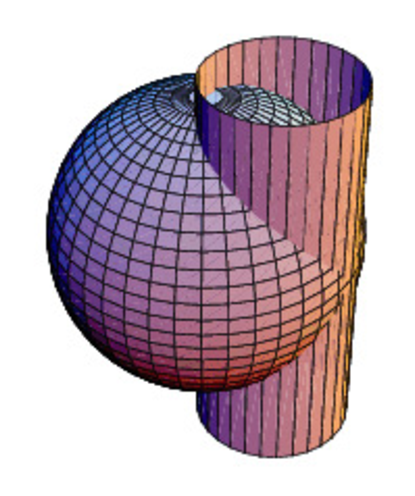
\psfig{file=viviani.eps,width=5cm}
\]

\eej

\bej  Sea la curva $z=f(x)$ $x\in [\alpha ,\beta ]$ con $f$ y $\alpha $
positivos, girada alrededor del eje $z$. Mostrar que el área de la
superficie barrida es
\[
A=2\pi \int_\alpha ^\beta x\sqrt{1+(f^{\prime }(x))^2}\ dx
\]
Aplicar a la superficie dada en el ejercicio (2) item a) para calcular el
área del paraboloide elíptico con $1\le z\le 2$, y $a=b=1$.
\eej

\bej Sea $\mathcal C$ la curva
\[
\left\{
\begin{aligned}
&x=\cos^3\theta\\
&y=\mbox{sen}^3\,\theta
\end{aligned}\right.
\]
con $0\le\theta\le 2\pi$
en el plano
$xy$. Sea $S$ la superficie que se obtiene al girar la curva $\mathcal C$
 alrededor del eje $x$
\begin{enumerate}
\item[a).] Hallar una parametrización de $S$.
\item[b).] Hallar el área de $S$.
\end{enumerate}
\eej

\bej  Calcular $\int_Sxy\ dS$ donde $S$ es el borde del tetraedro con lados
$z=0$, $y=0$, $x+z=1$ y $x=y$.
\eej

\bej  Calcular $\int_S(x+y+z)dS$ donde $S$ es el borde de la bola unitaria,
es decir
\[
S=\{(x,y,z)/x^2+y^2+z^2=1\}
\]
\eej

\bej  Hallar la masa de una superficie esférica de radio $r$ tal que en
cada punto $(x,y,z)\in S$ la densidad de masa es igual a la distancia entre $%
(x,y,z)$ y el punto $(0,0,r)$.
\eej

\begin{definition} Decimos que una superficie  $\Su$ es orientable si hay una forma de elegir
en cada punto $P$ de $\Su$ un único versor normal $\nu(P)$ de modo que la función vectorial
que esta elección define sobre $\Su$ resulte continua.

Por ejemplo, si $\Su$ es un gráfico, $\Su:\ \,z=f(x,y)$, se puede elegir en todos los puntos un versor normal
que apunte hacia arriba (es decir, con componente $z$ positiva). Esta elección es continua en $\Su$.

Si $\Su$ es el borde de una región $\Omega\subset \R^3$ de tipos I, II o III, se puede elegir como $\nu(P)$ la normal
que apunta hacia afuera de $\Omega$.
\end{definition}

\begin{prop}\label{orient} Sea $\Su$ una superficie suave y $T:D\subset\R^2\to\R^3$ una parametrización regular de $\Su$.
Para cada $P\in\Su$, sea
\[
\nu(P)=\frac{T_u(u,v)\times T_v(u,v)}{\|T_u(u,v)\times T_v(u,v)\|},\quad\mbox{donde }(u,v)\mbox{ es tal que }P=T(u,v).
\]
Entonces, esta elección de versor normal orienta la superficie $\Su$. En este caso, decimos que $\Su$ está orientada por la parametrización
$T$.
\end{prop}

\begin{definition} Sea $\Su$ una superficie orientada por el versor normal $\nu(P)$. Sea $\mbox{\rm\bf F}$ un campo vectorial continuo
sobre $\Su$. Llamamos flujo de $\mbox{\rm\bf F}$ a través de $\Su$ a la integral
\[
\int_\Su {\mbox{\rm\bf F}}\cdot d{\mbox{\rm\bf S}} \ :\,=\int_\Su {\mbox{\rm\bf F}}\cdot\nu\,dS.
\]
\end{definition}

\begin{prop}\label{nodepen2} Sea $\Su$ una superficie suave orientada por la parametrización regular $T:D\subset\R^2\to\R^3$.
Sea $T_1:D_1\subset
\R^2\to\R^3$ una reparametrización de $T$ que preserva la orientación. Sea $\mbox{\rm\bf F}$ un campo vectorial continuo
sobre $\Su$. Entonces, el cálculo de $\int_\Su {\mbox{\rm\bf F}}\cdot d\,{\mbox{\rm\bf S}}$ da el mismo resultado cuando
se utiliza la parametrización $T$ o la parametrización $T_1$. Si $T_1$ invierte la orientación, los cálculos difieren sólo
en el signo.
\end{prop}

\bej Probar la Proposición \ref{nodepen2}.
\eej

\bej  Evaluar el flujo saliente del campo ${\bf F}(x,y,z)=(x,y,z)$ a
través de la superficie del cubo $[0,1]\times [0,1]\times [0,1]$.
\eej

\bej  Si la temperatura en un punto de $\R^3$ está dada por la
función $T(x,y,z)=3x^2+3z^2$, calcular el flujo de calor (es decir el
flujo del campo $-\nabla T$) a traves de la superficie $x^2+z^2=2$, $0\le
y\le 2$, orientada de forma que la normal en el punto $(0,0,\sqrt{2})$ sea
(0,0,1).
\eej

\bej  Sea $S$ la superficie de la esfera unitaria orientada según la normal
exterior. Sea ${\bf F}$ un campo vectorial y ${ F}_r$ su componente
radial. Probar que
\[
\int_S{\bf F}\cdot d\,{\bf S}=\int_0^{2\pi }\int_0^\pi F_r\text{\,sen\,}(\phi
)\,d\phi \, d\theta
\]
\eej

\bej  Sea $S$ la parte del cono $z^2=x^2+y^2$ con $z$ entre 1 y 2 orientada
con la normal apuntando hacia el exterior del cono. Calcular $\int_S{\bf F}%
\cdot d\,{\bf S}$ con ${\bf F}(x,y,z)=(x^2,y^2,z^2)$.
\eej

\bej  Sean $S$ una superficie orientada y $C$ una curva cerrada
simple que es el borde de $S$ con alguna de sus dos posibles
orientaciones. Verificar que si ${\bf F}$ es un campo gradiente
(${\bf F}=\nabla f$) entonces
\[
\int_S\big(\nabla \times {\bf F}\big)\cdot d\,{\bf S}=\int_C{\bf F}\cdot d\,{\bf s}
\]
\eej

\bej  Sea ${\bf F}(x,y,z)=(x,x^2,yx^2)$ que representa el campo de
velocidad de un fluido (velocidad medida en metros por segundo). Calcular
cuántos metros cúbicos de fluido por segundo cruzan el plano $xy$ a
través del cuadrado $0\le x\le 1,\ 0\le y\le 1$.
\eej

\end{document}